\chapter{Quasi-Newton Methods}
\label{chap:quasi-newton}

\section{Introduction}

\paragraph{Principle.}
The goal is to avoid computing the Hessian by using a symmetric positive definite matrix instead.

\paragraph{Scope of application.}
In this chapter, we focus on small to medium-sized problems. Indeed, these methods require solving linear systems; the issue of large problems is deferred to the next chapter, where such resolutions will be avoided.

\section{The BFGS Method}
\label{sec:bfgs}

The \textbf{Broyden, Fletcher, Goldfarb, Shanno} (BFGS) method is the most popular Quasi-Newton method.

Consider the following quadratic model of the objective function $f$ at iteration $k$:
\begin{equation}
    m_k(p) = f_k + \nabla f_k^\top p + \frac{1}{2} p^\top B_k p,
\end{equation}
where $B_k$ is a symmetric positive definite matrix that is updated at each iteration.

Note that the model satisfies the following consistency properties at $p=0$:
\begin{itemize}
    \item $m_k(0) = f_k = f(x_k)$
    \item $\nabla m_k(0) = \nabla f_k = \nabla f(x_k)$
\end{itemize}

The minimizer $p_k$ of the quadratic model $m_k$ is obtained by setting its gradient to zero:
\begin{equation}
    \nabla m_k(p_k) = \nabla f_k + B_k p_k = 0.
\end{equation}
This implies that the search direction is given by:
\begin{equation}
    p_k = -B_k^{-1} \nabla f_k.
\end{equation}

Once the direction $p_k$ is obtained, we perform a line search to determine the step size $\alpha_k$.

\section{The Davidon-Fletcher-Powell (DFP) Update Formula}
\label{sec:dfp}

Davidon (1959) proposed updating $B_k$ to account for the change in curvature that occurred since the last iteration.

Consider the new affine model at $x_{k+1}$:
\begin{equation}
    m_{k+1}(p) = f_{k+1} + \nabla f_{k+1}^\top p + \frac{1}{2} p^\top B_{k+1} p.
\end{equation}

What are reasonable requirements for updating $B_k$?

\subsection{The Secant Equation}

For example, the gradient of $m_{k+1}$ must coincide with the true gradient of $f$ at points $x_{k+1}$ and $x_k$.

\begin{enumerate}
    \item At $x_{k+1}$ (i.e., for $p=0$):
    \[ \nabla m_{k+1}(0) = \nabla f_{k+1}. \]
    This condition is verified by definition.

    \item At $x_k$ (i.e., for the inverse displacement $p = -\alpha_k p_k$):
    We want:
    \begin{equation}
        \nabla m_{k+1}(-\alpha_k p_k) = \nabla f_{k+1} + B_{k+1}(-\alpha_k p_k) = \nabla f_k.
    \end{equation}
\end{enumerate}

Let's rearrange this last equation:
\[
    B_{k+1} (\alpha_k p_k) = \nabla f_{k+1} - \nabla f_k.
\]

Let us introduce the vectors $s_k$ (displacement) and $y_k$ (change in gradient):
\begin{align}
    s_k &= x_{k+1} - x_k = \alpha_k p_k, \\
    y_k &= \nabla f_{k+1} - \nabla f_k.
\end{align}

We then obtain the \textbf{secant equation}:
\begin{equation}
    \label{eq:secant}
    B_{k+1} s_k = y_k.
\end{equation}
The matrix $B_{k+1}$ must transform $s_k$ into $y_k$.

\begin{figure}[H]
\centering
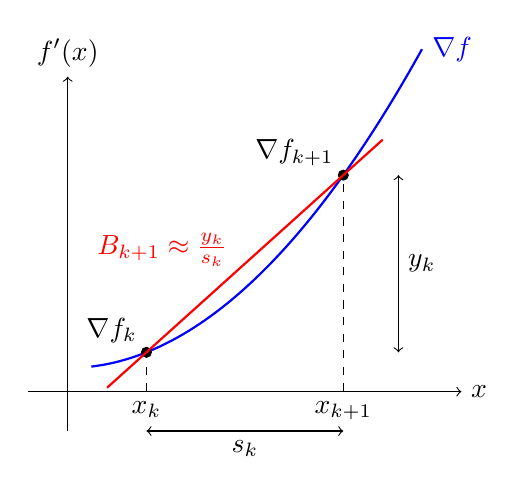
\begin{tikzpicture}[scale=1.0]
    % Axes
    \draw[->] (-0.5,0) -- (5,0) node[right] {$x$};
    \draw[->] (0,-0.5) -- (0,4) node[above] {$f'(x)$};
    
    % Derivative curve f'(x) - convex increasing: f'(x) = 0.2*x^2 + 0.3
    % At x=1: f'(1) = 0.2*1 + 0.3 = 0.5
    % At x=3.5: f'(3.5) = 0.2*12.25 + 0.3 = 2.45 + 0.3 = 2.75
    \draw[domain=0.3:4.5, smooth, variable=\x, blue, thick] 
        plot ({\x}, {0.2*\x*\x + 0.3}) node[right] {$\nabla f$};
    
    % Points x_k and x_{k+1}
    \coordinate (xk) at (1, 0);
    \coordinate (xk1) at (3.5, 0);
    \coordinate (fk) at (1, 0.5);
    \coordinate (fk1) at (3.5, 2.75);
    
    % Vertical lines to curve
    \draw[dashed] (1, 0) -- (fk);
    \draw[dashed] (3.5, 0) -- (fk1);
    
    % Points on curve
    \fill (fk) circle (2pt);
    \fill (fk1) circle (2pt);
    
    % Secant line - must pass through (1, 0.5) and (3.5, 2.75)
    % Slope = (2.75 - 0.5) / (3.5 - 1) = 2.25 / 2.5 = 0.9
    % At x=0.5: y = 0.5 + 0.9*(0.5 - 1) = 0.5 - 0.45 = 0.05
    % At x=4: y = 0.5 + 0.9*(4 - 1) = 0.5 + 2.7 = 3.2
    \draw[red, thick] (0.5, 0.05) -- (4, 3.2);
    
    % Labels
    \node[below] at (1, 0) {$x_k$};
    \node[below] at (3.5, 0) {$x_{k+1}$};
    \node[above left] at (fk) {$\nabla f_k$};
    \node[above left] at (fk1) {$\nabla f_{k+1}$};
    
    % Brace for s_k - lowered
    \draw[<->] (1, -0.5) -- (3.5, -0.5) node[midway, below] {$s_k$};
    
    % Brace for y_k
    \draw[<->] (4.2, 0.5) -- (4.2, 2.75) node[midway, right] {$y_k$};
    
    % Secant slope annotation - positioned upper left of red line
    \node[red] at (1.2, 1.8) {$B_{k+1} \approx \frac{y_k}{s_k}$};
\end{tikzpicture}
\caption{Geometric interpretation of the secant equation (1D case): $B_{k+1}$ is the slope of the secant line to the $\nabla f$ curve.}
\label{fig:secant-geometry}
\end{figure}

\begin{figureexplanation}
Figure~\ref{fig:secant-geometry} illustrates the principle of the secant equation in 1 dimension. The matrix (here a scalar) $B_{k+1}$ corresponds to the slope of the secant line (in red) connecting the points $(\nabla f_k, x_k)$ and $(\nabla f_{k+1}, x_{k+1})$ on the gradient curve (in blue). This slope approximates the average curvature of the function between these two points.
\end{figureexplanation}

\subsection{Curvature Condition}

A necessary condition for $B_{k+1}$ to be positive definite (as we want to ensure a descent direction) is obtained by multiplying the secant equation by $s_k^\top$ on the left:
\[
    s_k^\top B_{k+1} s_k = s_k^\top y_k.
\]
If $B_{k+1} \succ 0$, then we must have:
\begin{equation}
    s_k^\top y_k > 0.
\end{equation}
This is called the \textbf{curvature condition}.

\begin{itemize}
    \item This condition is always satisfied if $f$ is strongly convex.
    \item Otherwise, we must impose it by enforcing the \textbf{Wolfe conditions} during the line search.
\end{itemize}

\subsubsection{Proof using the Wolfe conditions}

The second Wolfe condition is:
\begin{equation}
    \nabla f_{k+1}^\top p_k \ge c_2 \nabla f_k^\top p_k.
\end{equation}
Since $s_k = \alpha_k p_k$ with $\alpha_k > 0$, this is equivalent to:
\[
    \nabla f_{k+1}^\top s_k \ge c_2 \nabla f_k^\top s_k.
\]
Thus:
\begin{align*}
    y_k^\top s_k
    &= (\nabla f_{k+1} - \nabla f_k)^\top s_k \\
    &\ge c_2 \nabla f_k^\top s_k - \nabla f_k^\top s_k \\
    &= (c_2 - 1) \nabla f_k^\top s_k \\
    &= (c_2 - 1) \alpha_k \nabla f_k^\top p_k.
\end{align*}
Since $c_2 < 1$ (hence $c_2 - 1 < 0$) and $p_k$ is a descent direction ($\nabla f_k^\top p_k < 0$), the product is strictly positive:
\[
    y_k^\top s_k > 0.
\]

\subsection{Construction of the DFP Update}

The secant equation $B_{k+1} s_k = y_k$ admits infinitely many solutions (because $B_{k+1}$ has $n(n+1)/2$ degrees of freedom for only $n$ constraints).

We need another criterion: choose $B_{k+1}$ to be as "close" as possible to $B_k$.
We solve:
\begin{equation}
    B_{k+1} = \arg\min_B \|B - B_k\| \quad \text{s.t. } B=B^\top \text{ and } B s_k = y_k.
\end{equation}

DFP chose the weighted Frobenius norm:
\[
    \|A\|_W = \|W^{1/2} A W^{1/2}\|_F, \quad \text{where } \|C\|_F^2 = \sum_{i,j} C_{ij}^2.
\]
The weighting matrix $W$ is chosen such that $W y_k = s_k$.

For instance, one can set $W = (\bar{G}_k)^{-1}$, where $\bar{G}_k$ is the average Hessian:
\[
    \bar{G}_k = \int_0^1 \nabla^2 f(x_k + \tau \alpha_k p_k) d\tau.
\]
By Taylor's theorem:
\[
    \nabla f(x_{k+1}) = \nabla f(x_k) + \bar{G}_k (x_{k+1} - x_k),
\]
which means $y_k = \bar{G}_k s_k$, verifying the choice of $W$.

With this choice of $W$, the solution is given by the DFP update formula:
\begin{equation}
    \label{eq:dfp-formula}
    B_{k+1} = (I - \rho_k y_k s_k^\top) B_k (I - \rho_k s_k y_k^\top) + \rho_k y_k y_k^\top,
\end{equation}
where
\begin{equation}
    \rho_k = \frac{1}{y_k^\top s_k}.
\end{equation}

\subsection{Expression for the Inverse (Sherman-Morrison-Woodbury Formula)}

If we express the update in terms of the inverse Hessian $H_k = B_k^{-1}$, as in Newton's method where $p_k = -H_k \nabla f_k$, we can use the Sherman-Morrison-Woodbury formula.

The DFP update formula for the inverse is given by:
\begin{equation}
    H_{k+1}^{DFP} = H_k - \frac{H_k y_k y_k^\top H_k}{y_k^\top H_k y_k} + \frac{s_k s_k^\top}{y_k^\top s_k}.
\end{equation}
We note that this update corresponds to adding two rank-1 matrices (a rank-2 update).
Furthermore, $\text{rank}(H_{k+1} - H_k) \le 2$.

\section{The BFGS Approach}
\label{sec:bfgs_approach}

The BFGS (Broyden-Fletcher-Goldfarb-Shanno) method uses the same reasoning as DFP, but works directly on the inverse Hessian $H_k$ instead of $B_k$.

The secant equation for the inverse becomes:
\begin{equation}
    H_{k+1} y_k = s_k.
\end{equation}
We then look for $H_{k+1}$ solving:
\begin{equation}
    H_{k+1} = \arg\min_H \|H - H_k\|_W \quad \text{s.t. } H=H^\top \text{ and } H y_k = s_k.
\end{equation}
The solution yields the \textbf{BFGS update formula} for the inverse:
\begin{equation}
    H_{k+1}^{BFGS} = (I - \rho_k s_k y_k^\top) H_k (I - \rho_k y_k s_k^\top) + \rho_k s_k s_k^\top,
\end{equation}
with $\rho_k = \frac{1}{y_k^\top s_k}$.

\begin{algorithm}[H]
\caption{BFGS Method}
\label{alg:bfgs}
Given starting point $x_0$, convergence tolerance $\varepsilon > 0$, inverse Hessian approximation $H_0$\;
$k \leftarrow 0$\;
\While{$\|\nabla f_k\| > \varepsilon$}{
    Compute search direction $p_k = -H_k \nabla f_k$\;
    Set $x_{k+1} = x_k + \alpha_k p_k$, where $\alpha_k$ is computed from a line search procedure to satisfy the Wolfe conditions\;
    $s_k \leftarrow x_{k+1} - x_k$\;
    $y_k \leftarrow \nabla f_{k+1} - \nabla f_k$\;
    Compute $H_{k+1} = (I - \rho_k s_k y_k')H_k(I - \rho_k y_k s_k') + \rho_k s_k s_k'$\;
    $k \leftarrow k + 1$\;
}
\end{algorithm}

\begin{figure}[H]
\centering

\includegraphics[width=0.7\textwidth]{4.png}
\caption{Iterations of the BFGS method on the level curves of the Rosenbrock function.}
\label{fig:bfgs-rosenbrock}
\end{figure}

\begin{figureexplanation}
\textbf{Key points to observe:}
\begin{itemize}
    \item \textbf{Direct trajectory:} Unlike gradient descent which zigzags, BFGS converges rapidly towards the minimum $(1,1)$ by using the curvature approximation.
    \item \textbf{Local adaptation:} The method progressively learns the shape of the Hessian over the iterations, allowing it to "straighten" its search directions.
    \item \textbf{Comparison:} The number of iterations is much lower than that of gradient descent (corresponding Figure in Chapter 2), but slightly higher than Newton (which uses the true Hessian).
\end{itemize}
\end{figureexplanation}

\section{Limited-Memory Quasi-Newton Methods (L-BFGS)}
\label{sec:lbfgs}

For high-dimensional problems, storing the matrix $H_k$ (of size $n \times n$) becomes prohibitive.
The L-BFGS (Limited-memory BFGS) method solves this problem by storing only the last $m$ pairs $(s_k, y_k)$.

\begin{algorithm}[H]
\caption{L-BFGS two-loop recursion}
\label{alg:lbfgs-twoloop}
$q \leftarrow \nabla f_k$\;
\For{$i = k-1, k-2, \ldots, k-m$}{
    $\alpha_i \leftarrow \rho_i s_i' q$\;
    $q \leftarrow q - \alpha_i y_i$\;
}
$r \leftarrow H_k^0 q$\;
\For{$i = k-m, k-m+1, \ldots, k-1$}{
    $\beta \leftarrow \rho_i y_i' r$\;
    $r \leftarrow r + s_i(\alpha_i - \beta)$\;
}
\Stop with result $H_k \nabla f_k = r$.
\end{algorithm}

\begin{algorithm}[H]
\caption{L-BFGS}
\label{alg:lbfgs}
Choose starting point $x_0$, integer $m > 0$\;
$k \leftarrow 0$\;
\Repeat{convergence}{
    Choose $H_k^0$, for instance $H_k^0 = \dfrac{s_{k-1}'y_{k-1}}{y_{k-1}'y_{k-1}} I$\;
    Compute $p_k \leftarrow -H_k \nabla f_k$ from Algorithm~\ref{alg:lbfgs-twoloop}\;
    Compute $x_{k+1} \leftarrow x_k + \alpha_k p_k$, where $\alpha_k$ is chosen to satisfy the Wolfe conditions\;
    \If{$k > m$}{
        Discard the vector pair $\{s_{k-m}, y_{k-m}\}$ from storage\;
    }
    Compute and save $s_k \leftarrow x_{k+1} - x_k$, $y_k = \nabla f_{k+1} - \nabla f_k$\;
    $k \leftarrow k + 1$\;
}
\end{algorithm}

\section{Remarks and Properties}

\paragraph{Initialization.} There is no universal optimal initialization for $H_0$.
The possibilities are:
\begin{itemize}
    \item Approximate the initial inverse Hessian.
    \item Take a multiple of the identity $H_0 = \gamma I$.
\end{itemize}

\paragraph{Cost.} The computational cost of each iteration is $O(n^2)$ (matrix-vector multiplications and rank 1/2 updates), as opposed to $O(n^3)$ for Newton (which requires a system inversion).

\paragraph{Positive Definiteness.}
If $H_k$ is positive definite, then $H_{k+1}$ is too, provided that $y_k^\top s_k > 0$.
Indeed, for any $z \neq 0$:
\[
    z^\top H_{k+1} z = z^\top (I - \rho s y^\top) H (I - \rho y s^\top) z + \rho (z^\top s)^2 \geq 0.
\]
Strictly speaking, at this stage we only have $\geq 0$ because $(I - \rho y s^\top) z$ and $z^\top s$ could be zero. However, if $z^\top s = 0$, then only the term $z^\top (I - \rho s y^\top) H (I - \rho y s^\top) z$ remains, which is $> 0$ because $H$ is positive definite and $(I - \rho y s^\top) z \neq 0$ (otherwise $z = \rho (y^\top z) s$, which would imply $z^\top s = \rho (y^\top z) s^\top s \neq 0$, a contradiction). Thus $z^\top H_{k+1} z > 0$.

\section{The Broyden Class}

There is a family of updates, called the Broyden class, defined by:
\begin{equation}
    B_{k+1} = (1-\phi_k) B_{k+1}^{BFGS} + \phi_k B_{k+1}^{DFP}.
\end{equation}
Or in explicit form:
\begin{equation}
    B_{k+1} = B_k - \frac{B_k s_k s_k^\top B_k}{s_k^\top B_k s_k} + \frac{y_k y_k^\top}{y_k^\top s_k} + \phi_k (s_k^\top B_k s_k) v_k v_k^\top,
\end{equation}
where $\phi_k$ is a scalar parameter and
\[
    v_k = \frac{y_k}{y_k^\top s_k} - \frac{B_k s_k}{s_k^\top B_k s_k}.
\]

Special cases:
\begin{itemize}
    \item If $\phi_k = 0$, we recover \textbf{BFGS}.
    \item If $\phi_k = 1$, we recover \textbf{DFP}.
\end{itemize}

\paragraph{Restricted Broyden Class.}
The restricted Broyden class corresponds to the choice $\phi_k \in [0, 1)$.
The methods in this class are convex combinations of BFGS and DFP.

\section{Properties on Quadratic Functions}

Consider a strongly quadratic function $f(x) = \frac{1}{2} x^\top Q x - b^\top x$.
Assume that $B_0$ is symmetric positive definite and that $\alpha_k$ is the exact step (exact line search).

Then we have the following properties (Admitted Theorem):
\begin{enumerate}
    \item The generated iterates $x_k$ are independent of the choice of $\phi_k$ in the Broyden class.
    \item The secant equation is satisfied for all previous search directions:
    \begin{equation}
        B_k s_j = y_j, \quad \forall j = 0, \dots, k-1.
    \end{equation}
    \item If we choose $B_0 = I$, then the iterates are identical to those of the conjugate gradient method, and the search directions are conjugate:
    \begin{equation}
        s_j^\top Q s_k = 0, \quad \forall j \neq k.
    \end{equation}
    \item If we perform $n$ iterations, then the Hessian matrix is identified exactly:
    \begin{equation}
        B_n = Q.
    \end{equation}
\end{enumerate}

\section{Convergence Analysis}

\subsection{Global Convergence}

\paragraph{Remark.}
BFGS and restricted Broyden class methods ($\phi_k \in [0, 1)$) are very robust in practice.
However, there is no global convergence result for general nonlinear (non-convex) functions.

We will state a result for convex functions.

\paragraph{Assumptions B.}
\begin{itemize}
    \item The objective function $f$ is twice continuously differentiable ($C^2$).
    \item The level set $\mathcal{L} = \{ x \in \mathbb{R}^n \mid f(x) \le f(x_0) \}$ is convex.
    \item There exist constants $0 < m \le M$ such that for any $z \in \mathbb{R}^n$ and any $x \in \mathcal{L}$:
    \begin{equation}
        m \|z\|^2 \le z^\top \nabla^2 f(x) z \le M \|z\|^2.
    \end{equation}
\end{itemize}
This implies that $f$ is strongly convex on $\mathcal{L}$.

\begin{theoreme}[Global Convergence of BFGS]
    Let $B_0$ be any symmetric positive definite matrix.
    Let $x_0$ be a point such that Assumptions B are verified.
    Then the sequence of iterates $(x_k)$ generated by the BFGS algorithm (with $\epsilon = 0$) converges to the minimizer $x^\star$ of $f$ (which is unique according to Assumptions B).
\end{theoreme}

\paragraph{Proof.} See \textit{\cite{nocedal2006numerical}}.

\paragraph{Remark.}
This theorem can be generalized to the entire restricted Broyden class.

\subsection{Superlinear Convergence of BFGS}

It is also possible to prove that the convergence is fast enough so that:
\[
    \sum_{k=0}^\infty \|x_k - x^\star\| < \infty.
\]

\paragraph{Assumption C.}
The Hessian matrix $G = \nabla^2 f$ is Lipschitz continuous at $x^\star$: there exists $L > 0$ such that for $x$ sufficiently close to $x^\star$:
\[
    \| \nabla^2 f(x) - \nabla^2 f(x^\star) \| \le L \| x - x^\star \|.
\]

\begin{theoreme}[Admitted]
    Suppose that $f$ is twice continuously differentiable ($C^2$).
    Consider the iterates $x_{k+1} = x_k + \alpha_k p_k$ where $\alpha_k$ satisfies the Wolfe conditions with $c_1 \le \frac{1}{2}$.
    If the sequence $(x_k)$ converges to a point $x^\star$ where $\nabla f(x^\star) = 0$ and $\nabla^2 f(x^\star)$ is positive definite.
    And if the search directions satisfy the Dennis-Moré condition:
    \begin{equation}
        \lim_{k \to \infty} \frac{\| \nabla f_k + \nabla^2 f_k p_k \|}{\| p_k \|} = 0,
    \end{equation}
    then the value $\alpha_k = 1$ is admissible for all $k \ge k_0$ (where $k_0$ is a certain integer),
    and if one chooses $\alpha_k = 1$ for $k \ge k_0$, the convergence of $(x_k)$ to $x^\star$ is \textbf{superlinear}.
\end{theoreme}

\paragraph{Remark.}
If $p_k = -B_k^{-1} \nabla f_k$ is a quasi-Newton direction, then the above condition rewrites as:
\[
    \lim_{k \to \infty} \frac{\| (B_k - \nabla^2 f(x_k)) p_k \|}{\| p_k \|} = 0.
\]
\bigskip
\begin{checkpoint}
\begin{itemize}
    \item \textbf{Secant Equation:} What relation must $B_{k+1}$ (or $H_{k+1}$) satisfy with respect to $s_k$ and $y_k$?
    \item \textbf{BFGS vs DFP:} Which method is the most robust in practice?
    \item \textbf{Limited Memory:} How does L-BFGS reduce the space complexity from $O(n^2)$ to $O(mn)$?
    \item \textbf{Convergence:} How fast does BFGS converge (Superlinear)?
\end{itemize}
\end{checkpoint}
